\chapter{Implementation}
\label{ch:implementation}

\section{Decisions}
\subsection{OS}
The backend and model inference services run on \textbf{Linux}. It provides stable CUDA and PyTorch support for GPU acceleration, lowering resource consumption for long-running services, and better compatibility with our model stack (LLM, ComfyUI, FastAPI). Linux is also widely adopted in AI production environments, which aligns with our deployment needs.

\subsection{Frontend Language}
We chose \textbf{Vue 3} as our frontend language. It provides a reactive system that helps update the interface automatically when data changes, which fits well with our project features like clothing display and recommendation results. The component-based design also makes it easier to manage the code and extend the system.

Vue also works well with UniApp, which is useful for supporting multiple platforms without rewriting the frontend. Although React is more popular and has a larger ecosystem, it often relies on additional third-party libraries for state management, which can increase development complexity \citep{Kari2024ComparisonOJ}. Considering the size of our project and our team’s experience, Vue was a more suitable choice.


\subsection{Backend Language}
The backend and AI modules are developed using \textbf{Python} with \textbf{FastAPI}. FastAPI is built on an Asynchronous Server Gateway Interface (ASGI), which supports non-blocking I/O and efficient concurrent request handling \citep{FastAPI2018}. This is important in our system, where AI inference tasks can take a relatively long time. By adopting asynchronous processing, the backend remains responsive and can handle multiple user requests without being blocked by long-running GPU inference.

We also considered Java frameworks (e.g. Spring Boot), which are widely used for scalable backend systems. However, integrating AI models in Java often requires additional service layers or external interfaces, which increases system complexity. In comparison, Python provides more direct support for AI workflows, making it more suitable for a system that heavily relies on model inference.



\subsection{Hardware}
This system relies on a high-performance GPU (\textbf{RTX 5090-level with 32GB VRAM}) to support virtual try-on generation. When the device first runs the virtual try on module, it takes about 32 seconds to load the model into GPU memory. After loading, each image generation takes approximately 10 seconds. This allows the system to provide users with relatively smooth interactions.

We also tested the system on a lower-end GPU (RTX 4060 with 8GB VRAM). In this case, the generation time increased to several minutes per image, and the output quality was significantly worse. 

Overall, these results show that the system has relatively high hardware requirements.

\subsection{Software}
\textbf{\large ComfyUI:}\\[0.4cm]
We selected ComfyUI as the runtime environment for image generation and virtual try-on features, mainly because of its modular workflow design and visual pipeline management. This makes the process easier to reproduce and allows more flexible control over model execution, which is helpful during debugging.

We also tried deploying the models directly. However, due to network restrictions, the offline installation process was not reliable. As a result, we adopted a solution based on the ComfyUI platform, combined with backend API calls, to implement the virtual try-on functionality.\\


\textbf{\large UniApp:}\\[0.4cm]
We chose UniApp for cross-platform development. Instead of building separate versions for web, mobile, and WeChat mini-programs, UniApp allows us to use a single codebase based on Vue3 and compile it for different platforms, which significantly reduces development and maintenance effort.

We also considered developing native applications for each platform. However, this would require more time and resources, and it would be difficult to maintain consistency of the user interface between platforms. In comparison, UniApp provides a relatively more efficient solution that enables a unified development process and consistent user experience while still meeting basic performance requirements.


\subsection{Supporting Tools}
\begin{itemize}
\item \textbf{Figma} was used to design interactive UI prototypes and simulate user flows.
\item \textbf{DrawIO} was used to create high-level system architecture diagrams and module composition visuals.
\item \textbf{Visual Paradigm} was used to draw UML diagrams. 
\end{itemize}


\subsection{Virtual Try-on Model}
\label{Chapter: Model Comparison and Selection}

\textbf{\large Qwen-Image-Edit}\\[0.4cm]
Figures \ref{fig:qwen-comparison} and \ref{fig:qwen-additional} demonstrate Qwen-Image’s editing performance. The model preserves the subject’s posture and background while generating new clothing with realistic material properties and shading, integrating it naturally into the original scene.

\begin{figure}[H]
  \centering
  \begin{minipage}{0.49\linewidth}
    \centering
    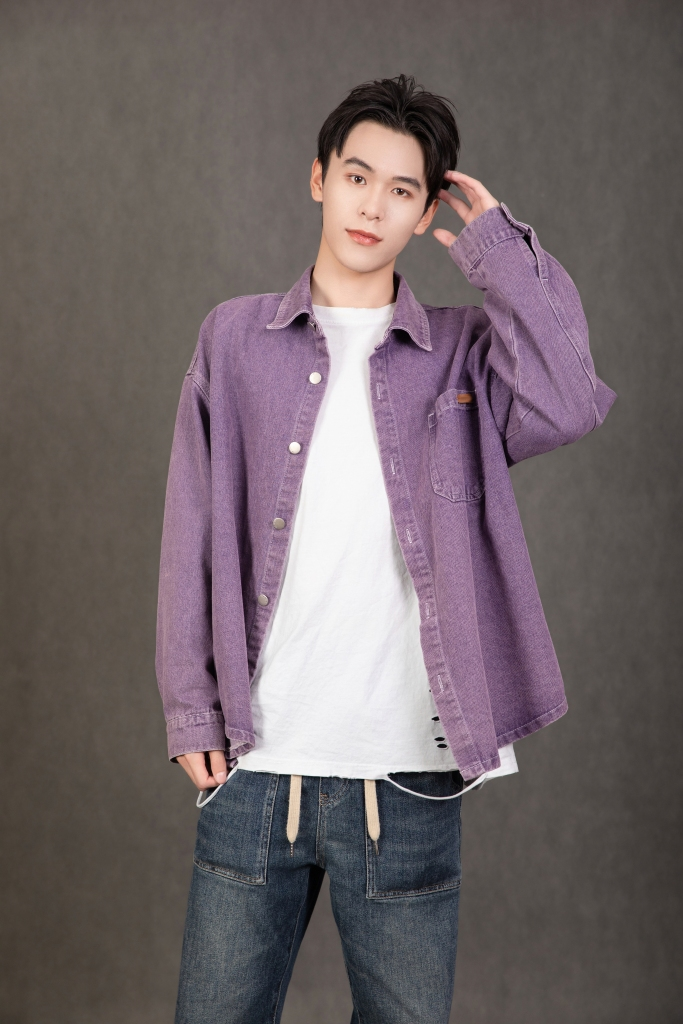
\includegraphics[width=\linewidth]{images/Section_6_Models/Qwen1.png}
    \caption{Original Body Image}
    \label{fig:qwen-comparison}
  \end{minipage}\hfill
  \begin{minipage}{0.49\linewidth}
    \centering
    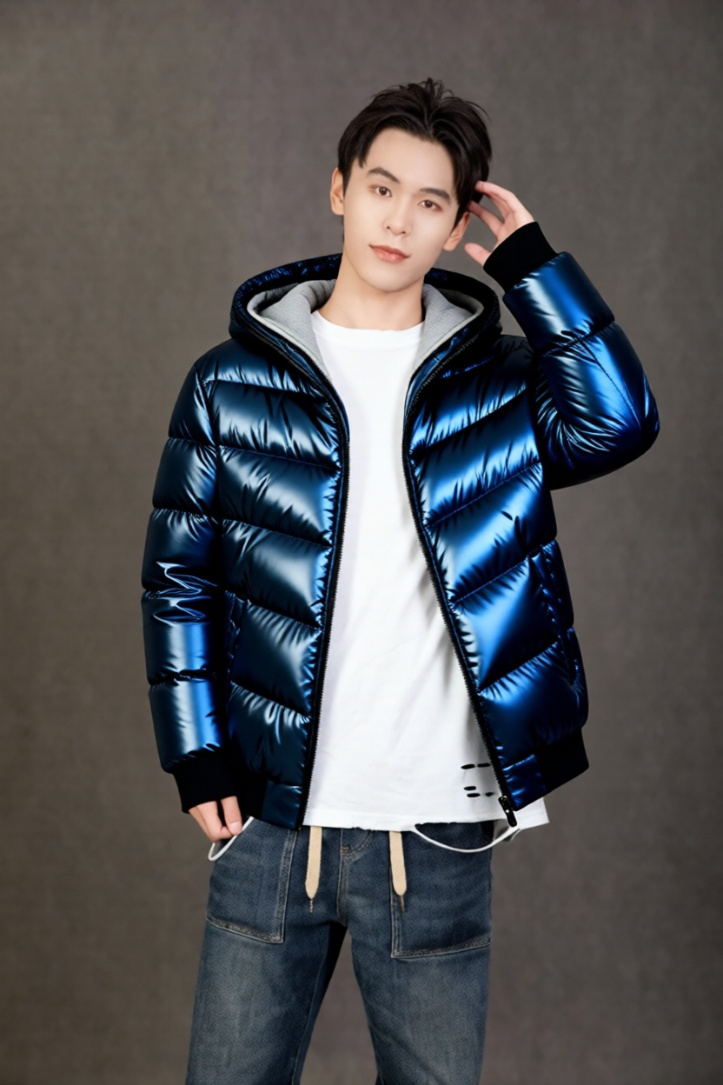
\includegraphics[width=\linewidth]{images/Section_6_Models/Qwen2.png}
    \caption{Qwen-Image-Edit Performance}
    \label{fig:qwen-additional}
  \end{minipage}
\end{figure}


\textbf{\large OOTDiffusion}\\[0.4cm]
Figures \ref{fig:ootd-comparison} and \ref{fig:ootd-additional} show OOTDiffusion’s performance. While the generated clothing is reasonably aligned with the body outline, the edited result shows noticeable deviations in arm posture and body proportions. In addition, subtle inconsistencies appear in local background regions, indicating that the model may alter non-target areas when handling complex clothing shapes or textures.

\begin{figure}[H]
  \centering
  \begin{minipage}{0.49\linewidth}
    \centering
    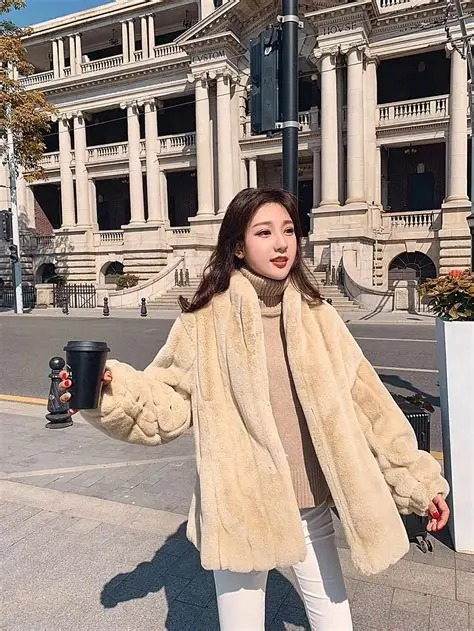
\includegraphics[width=\linewidth]{images/Section_6_Models/OOTD1.png}
    \caption{Original Body Image}
    \label{fig:ootd-comparison}
  \end{minipage}\hfill
  \begin{minipage}{0.49\linewidth}
    \centering
    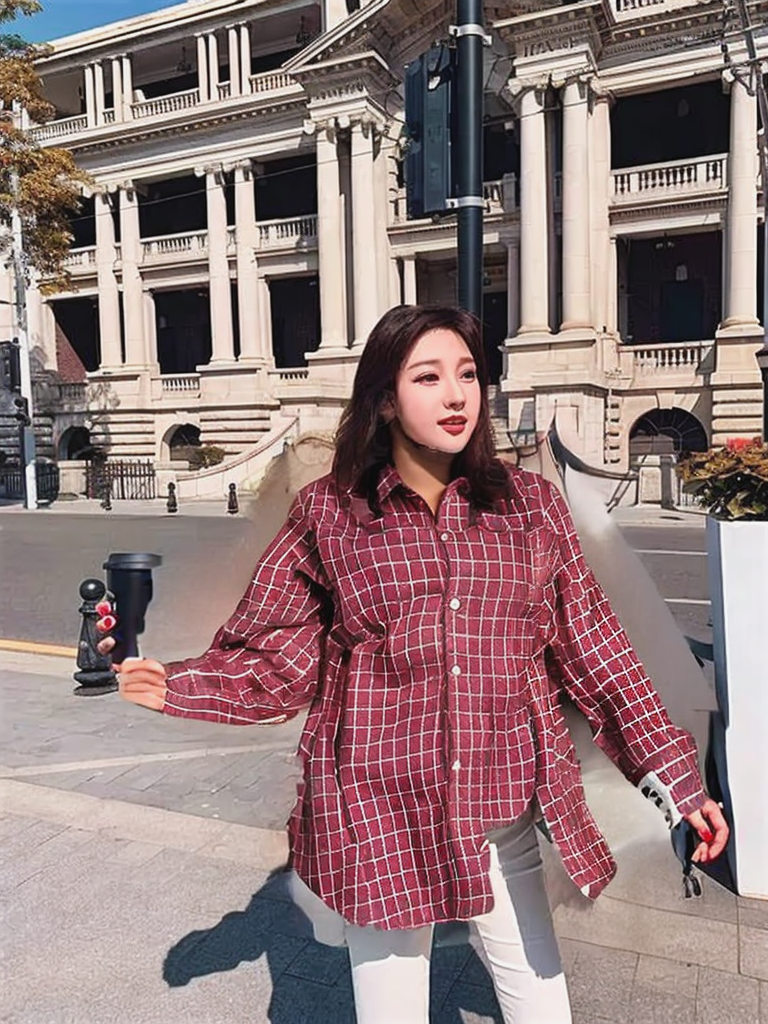
\includegraphics[width=\linewidth]{images/Section_6_Models/OOTD2.png}
    \caption{OOTD-Diffusion Performance}
    \label{fig:ootd-additional}
  \end{minipage}
\end{figure}


\noindent\textbf{\large Final Model Selection}
\vspace{0.4cm}

OOTDiffusion often applies overly large masks during garment replacement, which may distort backgrounds and fail to preserve fine-grained details such as jewelry or small accessories. In contrast, Qwen-Image-Edit better preserves posture, background, and local details while naturally integrating uploaded clothing (more examples provided in Appendix \ref{appendix: Qwen}).

As noted by \cite{hirakawa2026vtoniqa}, identity preservation and clothing consistency are key factors in virtual try-on quality. Thus, we determined that Qwen-Image-Edit would be the final model for our virtual try-on function.


\subsection{Recommendation Model}
\label{sec:llm_selection}
At the beginning of the project, we planned to deploy \textbf{gpt-oss} locally because it supports offline operation and has relatively low resource requirements, which theoretically reduces the dependence on external services. However, during the actual implementation process, we gradually found that only a few team members' device configurations could stably support the local deployment of this model. If consistent deployment cannot be achieved in all development environments, on the one hand, it will be difficult to ensure the reproducibility of system results, and on the other hand, it will also make development and debugging highly dependent on individual members, thus affecting overall development efficiency and collaboration stability.

Based on the aforementioned practical engineering constraints, we ultimately abandoned the local deployment plan and opted for \textbf{Qwen-Plus} as the core recommendation model. In comparison, Qwen-Plus provides stable inference services through a unified cloud interface, enabling all team members to develop and debug in a consistent environment. Additionally, this model excels in dialogue comprehension and semantic parsing, effectively supporting the mapping from natural language requirements to structured outfit recommendations.


\section{Results}
\subsection{Prototype}
This prototype implements all UI components defined in Chapter \ref{chapter_ui_design} and integrates them into a complete workflow. Each page corresponds to a core use case and provides seamless transitions across the user operation.

\begin{landscape}
\begin{figure}[H]
    \centering
    
\includegraphics[width=1.5\textwidth]{images/Section_6_Prototype/prototype.jpg}
    \caption{Prototype}
    \label{fig:Prototype}
\end{figure}
\end{landscape}


\subsection{Qwen-Image-Edit Model}
In this project, we decided to call the ComfyUI API to implement the virtual try-on functionality, and the implementation results are provided in Appendix \ref{appendix: Qwen}.

\textbf{\large ComfyUI Operation Procedure}

\begin{figure}[H]
    \centering
    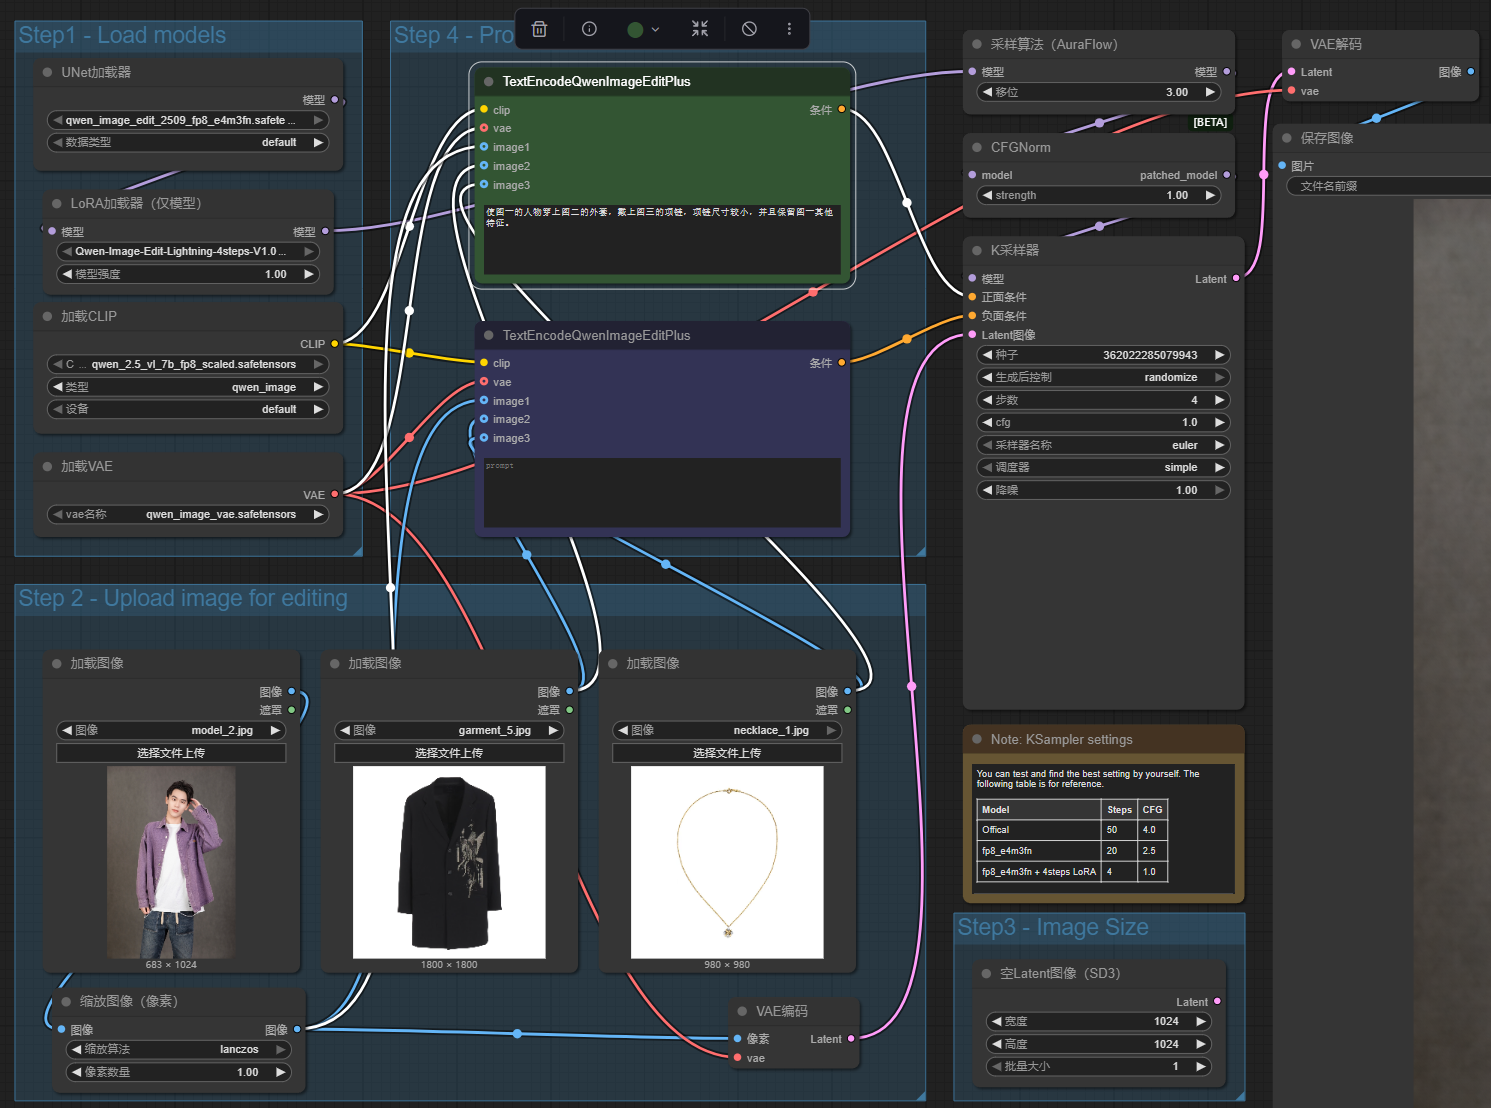
\includegraphics[width=0.95\textwidth]{images/Section_6.2.2/image.png}
    \caption{ComfyUI Workflow Interface for Qwen-Image-Edit}
    \label{fig:comfyui-detailed}
\end{figure}

\begin{enumerate}
    \item \textbf{Workflow Initialization}
    \begin{itemize}
        \item Open ComfyUI interface and load the pre-configured Qwen-Image-Edit workflow
        \item Ensure all necessary custom nodes are installed and updated
    \end{itemize}
    
    \item \textbf{Model Setup}
    \begin{itemize}
        \item Navigate to the model selection node and choose Qwen-Image-Edit
        \item Download necessary model components
        \item Check model compatibility and version requirements
    \end{itemize}
    
    \item \textbf{Input Configuration}
    \begin{itemize}
        \item In the image input nodes, upload:
        \begin{itemize}
            \item User reference photo (clear, full-body shot recommended)
            \item Clothing item image (front view, clean background)
            \item Accessory images if applicable (jewelry, shoes, etc.)
        \end{itemize}
        \item Adjust image preprocessing parameters if needed
    \end{itemize}
    
    \item \textbf{Generation Parameters}
    \begin{itemize}
        \item Set denoising strength (typically 0.7-0.9 for clothing try-on)
        \item Configure CFG scale for prompt adherence (recommended: 7.5-9.0)
        \item Adjust sampling steps for quality vs. speed balance
        \item Set random seed for reproducible results
    \end{itemize}
    
    \item \textbf{Execution and Monitoring}
    \begin{itemize}
        \item Click "Queue Prompt" to start generation
        \item Monitor progress in the execution queue
        \item Check console for any error messages or warnings
    \end{itemize}
    
    \item \textbf{Result Management}
    \begin{itemize}
        \item Review generated virtual try-on result
        \item Save output images
        \item Use API endpoints for automated batch processing
    \end{itemize}
\end{enumerate}

\newpage

\subsection{LLM}

This prototype implements the \textbf{LLM Recommendation} interface and shows how the recommendation module is integrated into the overall wardrobe assistant workflow. The page supports natural language interaction, presents outfit suggestions in a structured format, and explains the recommendation through item descriptions, styling rationale, and alternatives. It also links the results to downstream actions such as \textbf{virtual try-on}, \textbf{calendar scheduling}, and \textbf{look regeneration}, providing an interactive user experience.

\begin{figure}[H]
    \centering
    
\includegraphics[width=0.95\textwidth]{images/Section_6_Models/LLM.png}
    \caption{LLM interface}
    \label{fig:LLM}
\end{figure}


\begin{enumerate}
    \item \textbf{Natural Language Interaction}
    \begin{itemize}
        \item Users can describe outfit needs directly in conversational language
        \item The system interprets requests and returns personalized recommendations
    \end{itemize}

    \item \textbf{Structured Recommendation Display}
    \begin{itemize}
        \item Show the generated outfit title and overall style theme
        \item Present selected clothing items in a structured recommendation card
        \item Display style tags and brief semantic descriptions for each look
    \end{itemize}

    \item \textbf{Recommendation Explanation}
    \begin{itemize}
        \item Explain why the outfit works through styling rationale
        \item Provide warning messages for unsuitable pairings
        \item Offer alternative suggestions for comparison
    \end{itemize}

    \item \textbf{Downstream Interaction}
    \begin{itemize}
        \item Support item-level entry to the virtual try-on function
        \item Allow the complete outfit to be added to calendar scheduling
        \item Provide a look regeneration function for updated recommendations
    \end{itemize}
\end{enumerate}

\section{Implementation  Performance and Maturity}

The system implements most of the core functional requirements and supports the main workflow, including wardrobe management, AI recommendation, and virtual try-on.

To evaluate performance, several indicators were recorded during developing and testing. The results are shown in Table~\ref{tab:performance}.

\begin{table}[h]
\centering
\caption{Observed Performance Indicators by Module}
\begin{tabular}{lll}
\toprule
\textbf{Module} & \textbf{Task} & \textbf{Time} \\
\midrule

Wardrobe Management 
& Upload and auto-tag clothing 
& $\sim$5 s \\

\addlinespace

Virtual Try-On 
& Initial model loading and first generation 
& $\sim$32 s \\
& Subsequent try-on generation 
& $\sim$10 s \\
& Multiple clothing items 
& $\sim$10 s $\times$ n \\

\addlinespace

Recommendation AI 
& Text-only response 
& 6--7 s \\
& Structured recommendation output 
& 30--40 s \\
& Plan generation output 
& 40--50 s \\

\bottomrule
\end{tabular}
\label{tab:performance}
\end{table}

It can be seen that the system is fast for simple tasks such as wardrobe management and text responses. However, more complex features, such as virtual try-on and structured AI outputs, take longer due to model loading and processing.

From a usability point of view, most tasks can be completed in only a few steps, which meets the usability requirement. All core functions are able to run successfully, so the system can be considered a functional prototype.

However, the current implementation is not yet a production-ready application. The system depends on external AI services, which may cause delays or availability issues. In addition, although unit tests, integration tests, system tests and user acceptance tests were carried out (described in Chapter~\ref{ch:testing}), no stress tests or large-scale user tests have been conducted.

Therefore, further improvements are still needed before the implementation can be considered fully production-ready.